\documentclass[11pt,a4paper]{article}
\usepackage[T1]{fontenc}
\usepackage[utf8]{inputenc}
\usepackage[spanish,es-noshorthands,es-tabla]{babel}
\usepackage{amsmath,amssymb,bm}
\usepackage{graphicx,booktabs,hyperref,listings,geometry,enumitem,float}
\usepackage{siunitx}
\usepackage{subcaption}
\geometry{margin=2.4cm}
\graphicspath{{../../results/}}
\hypersetup{colorlinks=true,linkcolor=black,citecolor=blue,urlcolor=blue}
\lstset{
  language=Python,
  basicstyle=\ttfamily\footnotesize,
  breaklines=true,
  columns=fullflexible,
  frame=single,
  framesep=3pt,
  showstringspaces=false,
  commentstyle=\itshape,
  keepspaces=true,
  inputencoding=utf8,
  extendedchars=true,
  literate={á}{{\'a}}1 {é}{{\'e}}1 {í}{{\'i}}1 {ó}{{\'o}}1 {ú}{{\'u}}1
           {ñ}{{\~n}}1 {Á}{{\'A}}1 {μ}{{$\mu$}}1 {χ}{{$\chi$}}1 {ψ}{{$\psi$}}1
           {κ}{{$\kappa$}}1 {ω}{{$\omega$}}1 {θ}{{$\theta$}}1 {ε}{{$\varepsilon$}}1
           {Σ}{{$\Sigma$}}1 {π}{{$\pi$}}1 {²}{{$^2$}}1 {k̃}{{$\tilde k$}}1,
}
\newcommand{\dd}{\mathrm{d}}
\newcommand{\toep}[1]{[\![#1]\!]}
\newcommand{\kt}{\tilde k}
\newcommand{\code}[1]{\texttt{#1}}
\newcommand{\tabla}[1]{\IfFileExists{../../results/comparison/tables/#1.tex}%
  {\input{../../results/comparison/tables/#1.tex}}%
  {\textit{Tabla pendiente: ejecute scripts/comparison/run\_all.py.}}}
\IfFileExists{../../results/comparison/tables/efficiency_macros.tex}%
  {% Generado por scripts/comparison/efficiency.py: cifras de tiempo del anexo y del paper.
\providecommand{\EffAlpha}{2.52}
\providecommand{\EffAlphaShort}{2.5}
\providecommand{\EffProdBeta}{0.96}
\providecommand{\EffTmmRecMin}{0.23}
\providecommand{\EffTmmRecMax}{0.33}
\providecommand{\EffTmmScalar}{44}
\providecommand{\EffTmmMaxM}{20}
\providecommand{\EffTmmMaxLayers}{10\,946}
\providecommand{\EffProdFirst}{0.5}
\providecommand{\EffProdLast}{291}
\providecommand{\EffPweFirstM}{2}
\providecommand{\EffPweFirst}{3.3~ms}
\providecommand{\EffPweLastM}{10}
\providecommand{\EffPweLast}{32.5~s}
\providecommand{\EffPweGrowth}{3.4}
\providecommand{\EffExtrapAM}{12}
\providecommand{\EffExtrapA}{6~min}
\providecommand{\EffExtrapBM}{15}
\providecommand{\EffExtrapB}{3.7~h}
\providecommand{\EffExtrapBMem}{16~GB}
\providecommand{\EffMemEight}{19~MB}
\providecommand{\EffWpM}{5}
\providecommand{\EffWpTmmErr}{3\times10^{-15}}
\providecommand{\EffWpTmmMin}{1.4}
\providecommand{\EffWpTmmMax}{31}
\providecommand{\EffWpErrExp}{3.1}
\providecommand{\EffWpTimeExp}{2.5}
\providecommand{\EffWpTradeExp}{1.3}
\providecommand{\EffWpBestErr}{1\times10^{-6}}
\providecommand{\EffWpBestN}{385}
\providecommand{\EffWpBestTime}{1.2~s}
\providecommand{\EffWpSpeedRatio}{4\times10^{4}}
\providecommand{\EffWpErrRatio}{4\times10^{8}}
\providecommand{\EffWpTargetN}{3\times10^{4}}
\providecommand{\EffWpTargetMem}{68~GB}
\providecommand{\EffWpTargetTime}{23~h}
\providecommand{\EffFigTmmTotal}{0.32~s}
\providecommand{\EffFigPweTotal}{5.3~h}
\providecommand{\EffFigRatioMin}{2\times10^{4}}
\providecommand{\EffFigRatioMax}{4\times10^{5}}
\providecommand{\EffFigWallMin}{45}
\providecommand{\EffFigWallMax}{319}
\providecommand{\EffFigTmmMin}{2.9}
\providecommand{\EffFigTmmMax}{3.4}
\providecommand{\EffBookN}{101}
\providecommand{\EffBookPwe}{116~ms}
\providecommand{\EffBookTmm}{78~ms}
\providecommand{\EffBookGrid}{14~ms}
\providecommand{\EffBookGridPoints}{60\,001}
\providecommand{\EffBookErr}{5\times10^{-6}}
}{}

\title{El método de expansión en ondas planas para superredes de Fibonacci\\
con metamateriales dispersivos:\\
formulación, validación y comparación con la matriz de transferencia}
\author{Emanuel Orozco Gallego}
\date{28 de septiembre de 2026}

\begin{document}
\maketitle

\begin{abstract}
Se reformula el problema de Reyes-Gómez \textit{et al.}, Phys.\ Rev.\ B
\textbf{81}, 153101 (2010) ---bandas plasmón-polaritón en superredes de
Fibonacci aire/metamaterial--- con el método de expansión en ondas planas
(PWE, \textit{plane wave expansion}), siguiendo paso a paso el capítulo
unidimensional de Sukhoivanov y Guryev~\cite{sukhoivanov} y el cuaderno
\code{PWE-1d.ipynb} que lo acompaña. Primero se reproduce el ejemplo del libro
(cristal $\varepsilon_1=1$, $\varepsilon_2=9$): estructura de bandas, síntesis
de Fourier, perfil de campo y bandas fuera del eje con la condición de
Brewster. Después se muestra que la forma clásica $\omega(\mathbf{k})$ del PWE
no sirve para un metamaterial de Drude: el problema se vuelve cuadrático en
$\omega^2$ y aparecen autovalores espurios que se acumulan en la frecuencia de
plasma magnética. La solución adoptada es invertir los papeles y resolver
$k(\omega)$ como un problema cuadrático de autovalores, con la regla de
factorización inversa de Li~\cite{li1996}. Con ella la semitraza
$R_m=\cos(kL_m)$ del PWE coincide con la de la matriz de transferencia (TMM)
con errores de $10^{-7}$--$10^{-5}$ en la mayor parte del espectro (hasta
$\sim\!10^{-2}$ en el extremo de baja frecuencia, donde el contraste entre capas
llega a 400:1), los bordes de las subbandas de las Figs.~5--6
coinciden con errores relativos de ancho menores que $10^{-5}$ y el número de
subbandas sigue la regla $F_{m-2}$ del paper. Se documentan también los límites
del método: su costo $O(N^3)$ con $N\propto F_m$ y la aparición de bandas
espurias a menos de $\sim\!10^{-6}$~GHz de $\nu_m$, que se detectan y descartan
de forma automática. El anexo \textit{Comparación TMM vs PWE} reúne todas las
superposiciones y tablas de errores.
\end{abstract}

\tableofcontents
\newpage

%=====================================================================
\section{Introducción}
%=====================================================================

El PRB 2010 calcula la estructura de bandas de una superred cuya celda es la
palabra de Fibonacci $S_m$ ($S_0=B$, $S_1=A$, $S_{m}=S_{m-1}S_{m-2}$), formada por
capas de aire (A) y de un metamaterial (B) con respuesta de Drude
\begin{equation}
\varepsilon_B(\omega)=\varepsilon_0-\frac{\omega_e^2}{\omega^2},\qquad
\mu_B(\omega)=\mu_0-\frac{\omega_m^2}{\omega^2},
\label{eq:drude}
\end{equation}
con $a=b=\SI{12}{mm}$, $\omega_e/2\pi=\SI{3}{GHz}$ y
$\omega_m/2\pi=\SI{3}{GHz}$ (Figs.~1--2) o \SI{1}{GHz} (Figs.~3--6). El
resultado central es la semitraza $R_m=\tfrac12\operatorname{Tr}T_m=\cos(kL_m)$
de la matriz de transferencia de la celda: hay banda si $|R_m|\le 1$ y gap si
$|R_m|>1$. Justo debajo de $\nu_m=\omega_m/2\pi$ ($\mu_B\to 0^-$) aparecen
$F_{m-2}$ subbandas estrechas de plasmón-polaritón.

La implementación original del proyecto (\code{fibonacci\_photonics.solvers.tmm})
reproduce las seis figuras con la TMM. Este documento construye un segundo
método, independiente, basado en ondas planas, y lo usa para verificar esos
resultados. La TMM es exacta para medios estratificados (solo multiplica
matrices $2\times2$), así que el PWE no la sustituye; su valor está en que parte
de otra formulación (un problema de autovalores en el espacio recíproco) y, por
tanto, cualquier coincidencia entre ambos es una verificación fuerte.

\paragraph{Organización.} Las Secs.~\ref{sec:problema}--\ref{sec:algoritmo-libro}
siguen el orden del capítulo 4 del libro (4.1--4.11) aplicado a la celda $S_m$.
La Sec.~\ref{sec:benchmark} reproduce los resultados del libro (4.8, 4.9, 4.12).
La Sec.~\ref{sec:dispersivo} trata el caso dispersivo y la
Sec.~\ref{sec:kw} la formulación $k(\omega)$ que se usa en producción.
Las Secs.~\ref{sec:resultados}--\ref{sec:costo} presentan los resultados para
las Figs.~1--6 del paper, la convergencia y el costo. El
Apéndice~\ref{app:codigo} relaciona cada ecuación con el código.

%=====================================================================
\section{Planteamiento del problema}\label{sec:problema}
%=====================================================================

\subsection{Ecuación de onda en un medio estratificado}

El medio varía solo a lo largo de $z$ y la onda incide en el plano $xz$ con
componente tangencial conservada
\begin{equation}
q=\frac{\omega}{c}\,n_A\sin\theta,\qquad n_A=\sqrt{\varepsilon_A\mu_A}.
\end{equation}
Con dependencia $e^{i(qx-\omega t)}$, las ecuaciones de Maxwell se desacoplan en
dos polarizaciones. En TE ($\mathbf E=E_y\hat{\mathbf y}$) y en TM
($\mathbf H=H_y\hat{\mathbf y}$) la componente transversal $u(z)$ obedece la
misma ecuación
\begin{equation}
\boxed{\;\frac{\dd}{\dd z}\!\left[\frac{1}{\chi(z)}\frac{\dd u}{\dd z}\right]
+\left(\kappa^2\psi(z)-\frac{q^2}{\chi(z)}\right)u=0,\qquad \kappa=\frac{\omega}{c},\;}
\label{eq:onda}
\end{equation}
con
\begin{equation}
(u,\chi,\psi)=
\begin{cases}
(E_y,\;\mu,\;\varepsilon) & \text{TE},\\
(H_y,\;\varepsilon,\;\mu) & \text{TM}.
\end{cases}
\end{equation}
La ecuación~\eqref{eq:onda} es la versión estratificada del operador
$\hat\Theta=\nabla\times\varepsilon^{-1}\nabla\times$ de la ec.~(4.1) del libro,
que allí se escribe para $H$ con $\mu=1$ e incidencia normal. Las condiciones
en cada interfaz se leen directamente de la ecuación: $u$ y el \emph{flujo}
\begin{equation}
D(z)\equiv\frac{1}{\chi(z)}\frac{\dd u}{\dd z}
\label{eq:flujo}
\end{equation}
son continuos ($E_y$ y $H_x\propto\mu^{-1}\partial_zE_y$ en TE). Esta
observación, que en el libro no hace falta, será decisiva en la
Sec.~\ref{sec:factorizacion}.

\subsection{Teorema de Bloch}

Si $\chi$ y $\psi$ son periódicas con período $L$, las soluciones son funciones
de Bloch (ecs.~4.2 y 4.19 del libro)
\begin{equation}
u(z)=h(z)\,e^{ikz},\qquad h(z+L)=h(z),
\label{eq:bloch}
\end{equation}
y la relación de dispersión se expresa con la semitraza de la matriz de
transferencia de una celda, $T$:
\begin{equation}
\cos(kL)=\tfrac12\operatorname{Tr}T\equiv R.
\label{eq:semitraza}
\end{equation}
La TMM calcula $R$ multiplicando matrices $2\times2$; el PWE obtendrá $k$ (y por
tanto $R=\cos kL$) de un problema de autovalores. Ambas cantidades son la misma y
se pueden comparar punto a punto.

%=====================================================================
\section{Celda unidad y red directa}\label{sec:celda}
%=====================================================================

En el libro la celda unidad es una bicapa de espesores $a$ y $b$ (Fig.~4.2).
Aquí la celda es la palabra $S_m$ completa: $F_m$ capas con $F_{m-1}$ capas A y
$F_{m-2}$ capas B (con la indexación del paper, $F_0=F_1=1$), y período
\begin{equation}
L_m=F_{m-1}\,a+F_{m-2}\,b .
\end{equation}
La red directa es $R_\ell=\ell L_m$, $\ell\in\mathbb Z$ (ec.~4.7 con un solo
vector primitivo). La Tabla~\ref{tab:celdas} muestra el tamaño de las celdas
usadas. La superred es un cristal fotónico unidimensional ordinario con una
\emph{supercelda} cada vez más larga: la cuasiperiodicidad aparece solo en el
límite $m\to\infty$.

\begin{table}[H]
\centering
\caption{Celdas de Fibonacci usadas ($a=b=12$ mm).}
\label{tab:celdas}
\begin{tabular}{rlrrr}
\toprule
$m$ & $S_m$ & capas $F_m$ & capas B & $L_m$ (mm) \\
\midrule
2 & AB & 2 & 1 & 24 \\
3 & ABA & 3 & 1 & 36 \\
4 & ABAAB & 5 & 2 & 60 \\
5 & ABAABABA & 8 & 3 & 96 \\
6 & ABAABABAABAAB & 13 & 5 & 156 \\
7 & (21 capas) & 21 & 8 & 252 \\
\bottomrule
\end{tabular}
\end{table}

\noindent La palabra de cada orden la devuelve \code{physics.fibonacci.sequence(m)}
y es la misma en la TMM y en el PWE. La Fig.~\ref{fig:celda} muestra la celda
$S_4=\mathrm{ABAAB}$ y su perfil de permeabilidad.

%=====================================================================
\section{Red recíproca y zona de Brillouin}\label{sec:reciproca}
%=====================================================================

Toda función periódica de período $L_m$ se desarrolla en ondas planas con los
vectores de la red recíproca (ecs.~4.12--4.17)
\begin{equation}
G_n=\frac{2\pi n}{L_m},\qquad n\in\mathbb Z,
\qquad G_n R_\ell=2\pi n\ell .
\end{equation}
La primera zona de Brillouin es $-\pi/L_m<k\le\pi/L_m$. Como $L_m$ crece como
$F_m$, la zona se estrecha y las bandas de la celda bicapa se \emph{pliegan}
cada vez más: por eso el número de subbandas crece con $m$.

A partir de aquí todas las longitudes se adimensionalizan con $L_m$:
\begin{equation}
\kt=kL_m,\qquad \tilde G_n=G_nL_m=2\pi n,\qquad \tilde\kappa=\frac{\omega L_m}{c},
\qquad \tilde q=qL_m,
\label{eq:adim}
\end{equation}
de modo que la zona reducida es $|\mathrm{Re}\,\kt|\le\pi$ y $R=\cos\kt$.

%=====================================================================
\section{Desarrollo de Fourier de los perfiles}\label{sec:fourier}
%=====================================================================

\subsection{Coeficientes analíticos: generalización de la ec.~(4.38)}

Para un perfil constante por tramos, $f(z)=f_j$ en $[z_j,z_{j+1})$, con
$z_0=0<z_1<\dots<z_{F_m}=L_m$, los coeficientes
\begin{equation}
f_n=\frac1{L_m}\int_0^{L_m} f(z)\,e^{-iG_nz}\,\dd z
\end{equation}
son
\begin{equation}
f_0=\sum_j f_j\frac{d_j}{L_m},\qquad
f_n=\sum_{j} f_j\,\frac{i}{G_nL_m}\left(e^{-iG_nz_{j+1}}-e^{-iG_nz_j}\right),\quad n\neq0,
\label{eq:fourier}
\end{equation}
con $d_j=z_{j+1}-z_j$. Con dos capas ($z_1=a$, $z_2=a+b$) y $f=1/\varepsilon$ se
recupera exactamente la ec.~(4.38) del libro. Como en la superred cada capa es A
o B, basta con los coeficientes de las funciones indicadoras:
\begin{equation}
f_n=f_A\,(\mathbb 1_A)_n+f_B\,(\mathbb 1_B)_n .
\end{equation}
Con esto, para cada frecuencia los coeficientes de $\varepsilon(z)$, $\mu(z)$,
$1/\varepsilon$ o $1/\mu$ cuestan una combinación lineal de dos vectores
precalculados (\code{solvers.pwe.fourier.cell\_fourier}). Que $\varepsilon_B$ y
$\mu_B$ sean negativos o dependan de $\omega$ no cambia nada.

\subsection{Matrices de Toeplitz}

El producto de dos funciones periódicas se convierte en una convolución de
coeficientes. Truncando a $n=-n_{\max}\dots n_{\max}$ ($N=2n_{\max}+1$ ondas
planas) se representa con la matriz de Toeplitz
\begin{equation}
\toep{f}_{nn'}=f_{n-n'},
\label{eq:toeplitz}
\end{equation}
que necesita los coeficientes hasta $|n|=2n_{\max}$.

\subsection{Validación de la síntesis (Fig.~4.6 del libro)}

Antes de calcular bandas conviene sintetizar el perfil con los coeficientes y
compararlo con el original. La Fig.~\ref{fig:sintesis} reproduce la Fig.~4.6
del libro para $1/\varepsilon$ de la bicapa, y la Fig.~\ref{fig:celda} hace lo
mismo para $\mu(z)$ en la celda $S_4$. Se ven dos hechos que guían el resto del
trabajo: (i) los coeficientes decaen solo como $1/|n|$, por los saltos del
perfil; (ii) la síntesis presenta el fenómeno de Gibbs en cada interfaz, con un
sobreimpulso de $\sim\!9\%$ que no desaparece al aumentar $N$. En la superred
hay $F_m$ interfaces por celda, así que $N$ debe crecer con $F_m$ para mantener
la misma resolución por capa:
\begin{equation}
n_{\max}=h\,F_m,
\label{eq:truncamiento}
\end{equation}
con $h$ el número de armónicos por capa (entre 8 y 16 en este trabajo).

\begin{figure}[H]
\centering
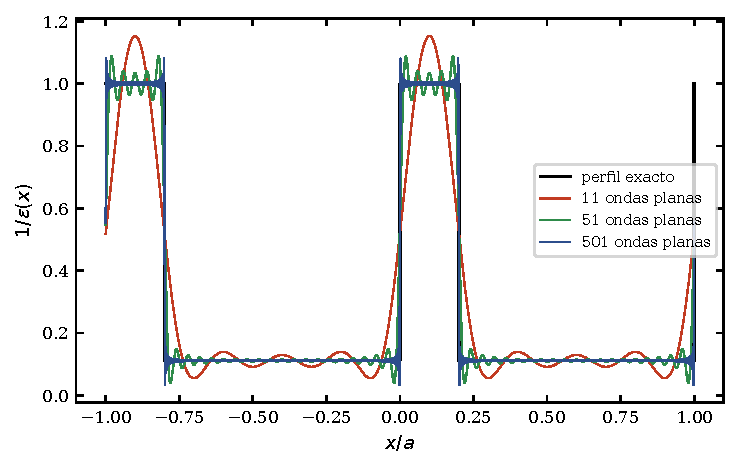
\includegraphics[width=0.72\linewidth]{pwe/book_benchmark/output/fourier_synthesis.pdf}
\caption{Síntesis de $1/\varepsilon(x)$ para la bicapa del libro
($\varepsilon_1=1$, $\varepsilon_2=9$, $l_1=0.2a$, $l_2=0.8a$) con 11, 51 y 501
ondas planas (equivalente a la Fig.~4.6 del libro). Los valores
$1/\varepsilon_1=1$ y $1/\varepsilon_2=1/9$ se reproducen ya con 11 ondas planas;
al aumentar $N$ solo mejora la forma cerca de los saltos.}
\label{fig:sintesis}
\end{figure}

\begin{figure}[H]
\centering
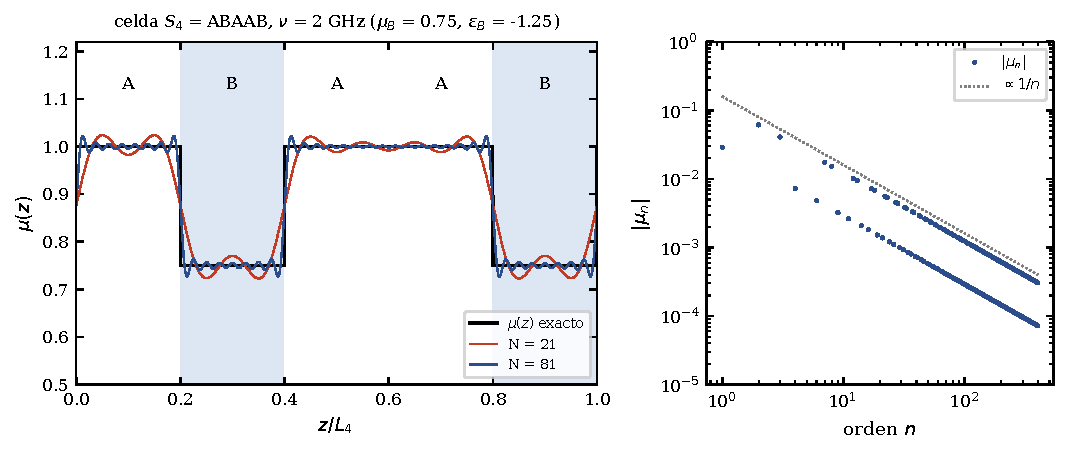
\includegraphics[width=\linewidth]{pwe/cell_fourier/output/cell_fourier.pdf}
\caption{Izquierda: perfil de permeabilidad de la celda $S_4$ a $\nu=2$~GHz
(parámetros de la Fig.~3 del paper, $\mu_B=0.75$) y su síntesis con
$N=21$ y $N=81$ ondas planas ($h=2$ y $h=8$). Derecha: módulo de los
coeficientes $\mu_n$; las dos ramas corresponden a órdenes con distinta
interferencia entre las cinco interfaces y ambas decaen como $1/n$.}
\label{fig:celda}
\end{figure}

%=====================================================================
\section{Ecuación maestra y problema de autovalores}\label{sec:maestra}
%=====================================================================

\subsection{Sustitución de la expansión}

Se sustituye en~\eqref{eq:onda} la función de Bloch desarrollada en ondas
planas (ec.~4.20)
\begin{equation}
u(z)=\sum_{n=-n_{\max}}^{n_{\max}}u_n\,e^{i(k+G_n)z}
\end{equation}
y los perfiles desarrollados según~\eqref{eq:fourier}. Proyectando sobre
$e^{i(k+G_n)z}$ y usando $K=\mathrm{diag}(k+G_n)$, la ecuación de onda se
convierte en el sistema lineal
\begin{equation}
K\,P\,K\,\mathbf u+q^2\toep{1/\chi}\,\mathbf u=\kappa^2\toep{\psi}\,\mathbf u ,
\label{eq:maestra}
\end{equation}
donde $P$ es la representación matricial de $1/\chi$ dentro del término de
flujo. En el caso del libro (TM, $\chi=\varepsilon$, $\psi=\mu=1$, $q=0$) y con
$P=\toep{1/\varepsilon}$, la ec.~\eqref{eq:maestra} es la \emph{master
equation} (4.25):
\begin{equation}
\sum_{G'}\chi(G-G')\,(k+G)(k+G')\,h(G')=\frac{\omega^2}{c^2}\,h(G),
\qquad \chi(G)=\left(\tfrac1\varepsilon\right)_G .
\end{equation}

\subsection{Hermiticidad y autovalores (Secs.~4.6--4.7)}

Para medios sin pérdidas y sin dispersión, $\toep{f}$ es hermítica porque
$f_{-n}=f_n^*$ para $f$ real, y $K$ es real y diagonal; por tanto
$A=KPK+q^2\toep{1/\chi}$ y $B=\toep{\psi}$ son hermíticas y $B$ es definida
positiva. La ec.~\eqref{eq:maestra} es un problema generalizado hermítico
$A\mathbf u=\lambda B\mathbf u$, con $\lambda=\kappa^2$ real y no negativo, que
se resuelve con \code{scipy.linalg.eigh} (Secs.~4.6--4.7 del libro). Cada $k$
de la zona de Brillouin da $N$ frecuencias; las más bajas convergen primero.

\subsection{Campo eléctrico frente a campo magnético (Sec.~4.10)}

El libro explica que la ecuación para $E$ con $\varepsilon$ no uniforme lleva a
una matriz no hermítica (ecs.~4.39--4.42). En la forma~\eqref{eq:maestra}
ese problema no aparece: el operador $K P K$ es siempre simétrico. Lo que cambia
entre polarizaciones es solo qué respuesta está dentro de la derivada
($\chi$) y cuál multiplica a $\kappa^2$ ($\psi$). En TE, $u=E_y$ y dentro de la
derivada queda $1/\mu$; en TM, $u=H_y$ y queda $1/\varepsilon$, como en el
libro.

\subsection{Propagación fuera del eje (Sec.~4.12)}

Con $q\neq0$ aparece el término $q^2\toep{1/\chi}$, equivalente a la ec.~(4.44)
del libro. La frecuencia mínima deja de ser cero y las bandas se estrechan al
crecer $q$. En TM, las bandas se cierran (``cinturas'') cuando la onda cruza las
interfaces con el ángulo de Brewster, porque no hay reflexión de Fresnel
(ec.~4.45):
\begin{equation}
q_B=\frac{\omega}{c}\,\frac{n_1n_2}{\sqrt{n_1^2+n_2^2}} .
\label{eq:brewster}
\end{equation}

%=====================================================================
\section{Algoritmo del PWE (Sec.~4.11)}\label{sec:algoritmo-libro}
%=====================================================================

Para medios no dispersivos el algoritmo del libro, aplicado a la celda $S_m$,
queda así:
\begin{enumerate}[label=\arabic*.]
\item Calcular los coeficientes de $\mathbb 1_A$ y $\mathbb 1_B$ con la
ec.~\eqref{eq:fourier} para $|n|\le 2n_{\max}$.
\item Recorrer $k$ en la zona de Brillouin, $-\pi/L_m\dots\pi/L_m$.
\item Usar $G_n$ entre $-2\pi n_{\max}/L_m$ y $2\pi n_{\max}/L_m$ ($N=2n_{\max}+1$
ondas planas).
\item Para cada $k$ armar $A$ y $B$ de la ec.~\eqref{eq:maestra} y calcular sus
autovalores $\lambda=\kappa^2$; $\omega=c\sqrt\lambda$.
\item Dibujar $\omega L_m/2\pi c$ frente a $k$.
\end{enumerate}
La implementación está en \code{solvers.pwe.eigenfrequency.nondispersive\_bands}; el
listado del Apéndice~\ref{app:codigo} muestra el núcleo.

%=====================================================================
\section{Validación con el cristal del libro}\label{sec:benchmark}
%=====================================================================

Se usan los parámetros del cuaderno \code{PWE-1d.ipynb}: $\varepsilon_1=1$,
$\varepsilon_2=9$, $l_1=0.2\,\mu$m, $l_2=0.8\,\mu$m ($a=l_1+l_2$) y
$n_{\max}=50$ ($N=101$). La referencia exacta es la TMM de la bicapa, que da
$\cos(ka)=\tfrac12\operatorname{Tr}T(\omega)$ en forma cerrada.

\subsection{Estructura de bandas (Fig.~4.5 del libro)}

La Fig.~\ref{fig:libro-bandas} superpone las ocho primeras bandas del PWE y la
curva exacta. Con la regla de Laurent que usa el libro
($P=\toep{1/\varepsilon}$) las bandas altas quedan ligeramente desplazadas: el
residuo máximo $|\cos(ka)-R_{\rm TMM}(\omega_{\rm PWE})|$ es $0.157$. Con la
regla inversa ($P=\toep{\varepsilon}^{-1}$, Sec.~\ref{sec:factorizacion}) baja a
$1.6\times10^{-4}$ con las mismas 101 ondas planas. La
Tabla~\ref{tab:libro-conv} muestra que la diferencia se mantiene a todo $N$:
Laurent converge como $N^{-1}$ y la regla inversa como $N^{-3}$.

\begin{figure}[H]
\centering
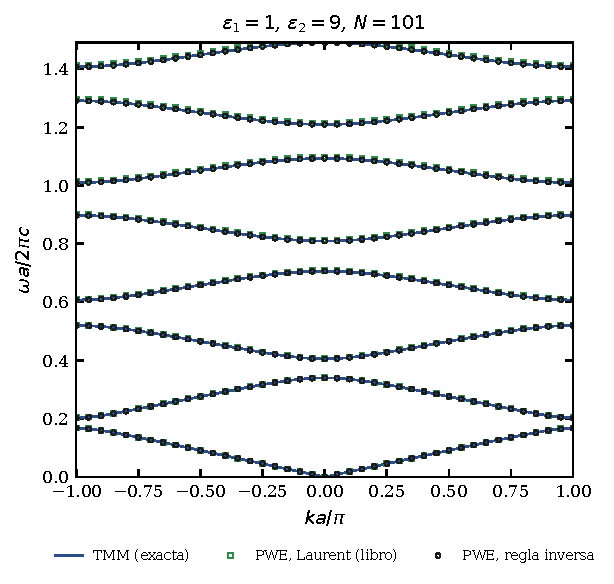
\includegraphics[width=0.62\linewidth]{pwe/book_benchmark/output/band_structure.pdf}
\caption{Estructura de bandas del cristal del libro. Línea: TMM exacta.
Cuadrados: PWE con la regla de Laurent (como en el libro). Círculos: PWE con la
regla inversa. $N=101$.}
\label{fig:libro-bandas}
\end{figure}

\begin{table}[H]
\centering
\caption{Error relativo máximo de las frecuencias de las cuatro primeras bandas del
cristal del libro en $ka/\pi=0.25,\,0.5,\,0.75$, frente a la TMM, según el número
de ondas planas.}
\label{tab:libro-conv}
\tabla{book_convergence}
\end{table}

\subsection{Perfil de campo}

El cuaderno dibuja la intensidad de un modo alto ($k=\pi/15a$, banda 11). Con
los autovectores $u_n$ se reconstruye $H(x)=\sum u_ne^{i(k+G_n)x}$
(Fig.~\ref{fig:libro-campo}). El campo oscila más rápido en la capa
$\varepsilon_2=9$, donde el índice es mayor, y es suave en la capa de aire.

\begin{figure}[H]
\centering
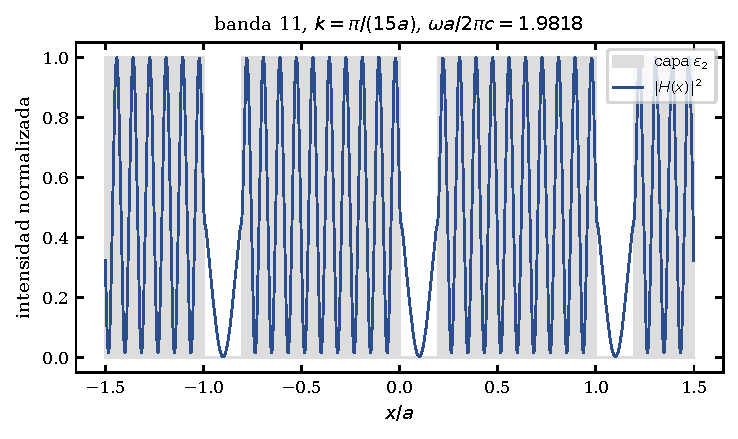
\includegraphics[width=0.72\linewidth]{pwe/book_benchmark/output/field_profile.pdf}
\caption{Intensidad $|H(x)|^2$ del modo de la banda 11 para $k=\pi/(15a)$ en
tres celdas. Las zonas sombreadas son las capas $\varepsilon_2=9$.}
\label{fig:libro-campo}
\end{figure}

\subsection{Diagrama proyectado fuera del eje (Fig.~4.9 del libro)}

Para cada $q$ se calculan las bandas en $k=0$ y $k=\pi/a$; entre ellas está la
banda permitida. La Fig.~\ref{fig:libro-offaxis} compara esos bordes con el mapa
exacto $|R_{\rm TMM}(\omega,q)|\le1$. En TE los gaps se ensanchan con $q$; en
TM se cierran exactamente sobre la recta de Brewster~\eqref{eq:brewster}, como
indica el libro.

\begin{figure}[H]
\centering
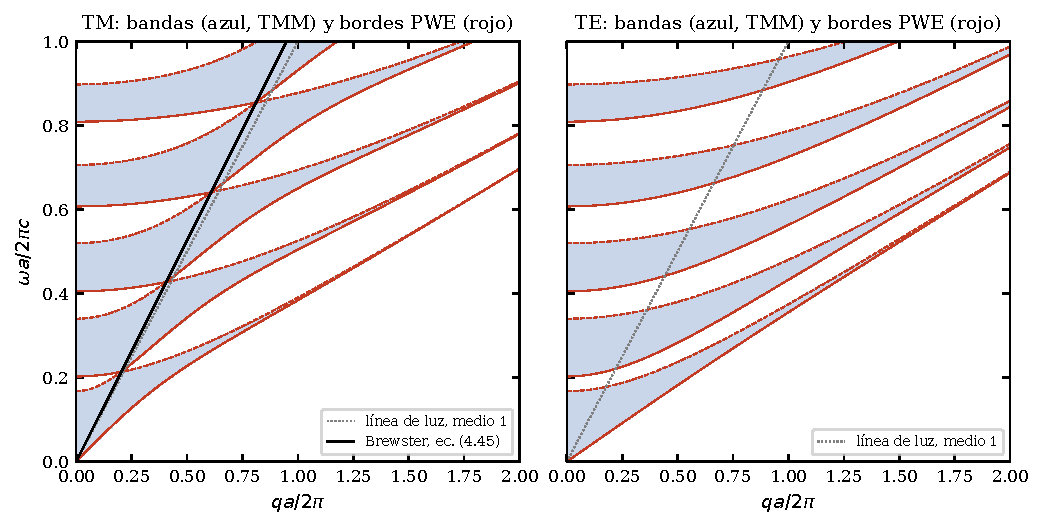
\includegraphics[width=\linewidth]{pwe/book_benchmark/output/off_axis_projected_bands.pdf}
\caption{Bandas proyectadas fuera del eje. Fondo azul: regiones permitidas
según la TMM. Líneas rojas: bordes del PWE ($k=0$ continuas, $k=\pi/a$ a
trazos, $N=61$). En TM (izquierda) las cinturas caen sobre la condición de
Brewster, ec.~(4.45).}
\label{fig:libro-offaxis}
\end{figure}

%=====================================================================
\section{Metamateriales dispersivos: por qué falla la forma $\omega(k)$}\label{sec:dispersivo}
%=====================================================================

\subsection{El problema cuadrático en $\omega^2$}

En la superred, $\varepsilon_B$ y $\mu_B$ dependen de $\omega$ según la
ec.~\eqref{eq:drude}, de modo que la ec.~\eqref{eq:maestra} ya no es un problema
lineal de autovalores. En TE, multiplicando la ecuación de onda por
$D(\lambda)=\mu_0\lambda-\lambda_m$ (con $\lambda=\tilde\kappa^2$,
$\lambda_{e,m}=(\omega_{e,m}L_m/c)^2$ y $\mu_B=D/\lambda$) todos los coeficientes
se vuelven polinomios en $\lambda$:
\begin{equation}
\frac{D}{\mu}=\lambda p_1+p_0,\qquad
D\left(\varepsilon-\frac{s^2}{\mu}\right)\lambda=\lambda^2r_2+\lambda r_1+r_0,
\qquad s^2=\varepsilon_A\mu_A\sin^2\theta,
\end{equation}
con, capa por capa,
\begin{align}
p_1&=\{\mu_0/\mu_A,\;1\}, & p_0&=\{-\lambda_m/\mu_A,\;0\},\\
r_2&=\{\alpha_A\mu_0,\;\varepsilon_0\mu_0-s^2\}, &
r_1&=\{-\alpha_A\lambda_m,\;-(\varepsilon_0\lambda_m+\mu_0\lambda_e)\}, &
r_0&=\{0,\;\lambda_e\lambda_m\},
\end{align}
y $\alpha_A=\varepsilon_A-s^2/\mu_A$. Se obtiene un problema cuadrático de
autovalores (QEP) en $\lambda$,
\begin{equation}
\left[\lambda^2M_2+\lambda M_1+M_0\right]\mathbf u=0,\qquad
M_2=\toep{r_2},\;M_1=\toep{r_1}-K\toep{p_1}K,\;M_0=\toep{r_0}-K\toep{p_0}K,
\label{eq:qep-omega}
\end{equation}
que se linealiza en forma compañera de tamaño $2N$~\cite{tisseur}
(función \code{drude\_qep\_frequencies\_ghz} de \code{solvers/pwe/eigenfrequency.py}).

\subsection{Contaminación espectral}

La Fig.~\ref{fig:contaminacion} resuelve~\eqref{eq:qep-omega} para $m=3$,
$\theta=\pi/12$ y $kL_m=\pi/2$ con $N=21\dots241$. La TMM da exactamente dos
frecuencias en la ventana 0.5--3~GHz (0.99852 y 2.80589~GHz). El QEP las
contiene, pero añade muchos autovalores espurios que no convergen al aumentar
$N$ (Tabla~\ref{tab:contaminacion}) y que se acumulan en $\nu_m$, a distancias
de $10^{-2}$ a $10^{-16}$~GHz. El origen es doble:
\begin{enumerate}[label=(\roman*)]
\item el término $K\toep{p_0}K$ contiene la función escalonada $D/\mu$, que se
anula en las capas B, y la regla de Laurent para un producto de dos funciones
discontinuas no converge (Sec.~\ref{sec:factorizacion});
\item cerca de $\mu_B=0$ el operador tiene un espectro esencial en $\nu_m$ (una
capa con $\mu\to0$ soporta infinitos modos localizados), que la discretización
aproxima con una nube de autovalores~\cite{tip}.
\end{enumerate}
Distinguir los autovalores físicos exige comprobarlos uno por uno con la TMM, lo
que anula la utilidad de la forma $\omega(k)$ para esta superred.

\begin{figure}[H]
\centering
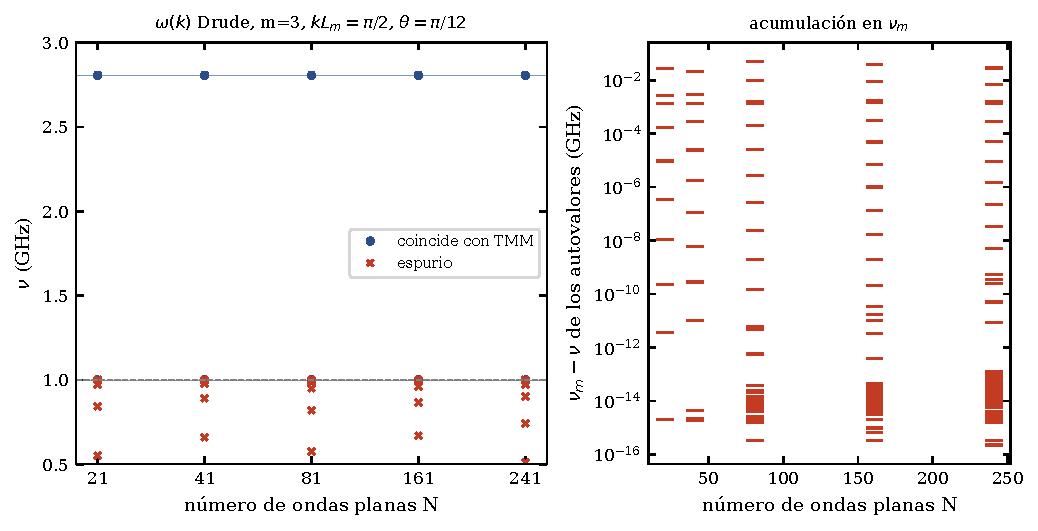
\includegraphics[width=\linewidth]{pwe/spectral_pollution/output/spectral_pollution.pdf}
\caption{Contaminación espectral de la forma $\omega(k)$ con Drude ($m=3$,
$kL_m=\pi/2$, $\theta=\pi/12$). Izquierda: autovalores reales en 0.5--3~GHz;
en azul los que coinciden con las raíces de la TMM (líneas horizontales), en
rojo los espurios. Derecha: distancia a $\nu_m$ de los autovalores situados
justo debajo; se acumulan hacia $\nu_m$ al crecer $N$.}
\label{fig:contaminacion}
\end{figure}

\begin{table}[H]
\centering
\caption{Autovalores del QEP~\eqref{eq:qep-omega} en la ventana 0.5--3~GHz y
cuántos no corresponden a ninguna raíz de la TMM.}
\label{tab:contaminacion}
\tabla{pollution}
\end{table}

%=====================================================================
\section{Formulación $k(\omega)$ con la regla inversa}\label{sec:kw}
%=====================================================================

\subsection{Reglas de factorización de Li}\label{sec:factorizacion}

El término de flujo $(1/\chi)\,u'$ es el producto de dos funciones discontinuas
en las interfaces cuyo producto $D$ es continuo, ec.~\eqref{eq:flujo}. Li
demostró~\cite{li1996} que para ese producto la regla de Laurent,
\begin{equation}
[D]\approx\toep{1/\chi}\,[u'],
\end{equation}
converge lentamente y a un valor incorrecto para $N$ finito, mientras que la
regla inversa,
\begin{equation}
[u']=\toep{\chi}\,[D]\;\Longrightarrow\;[D]\approx\toep{\chi}^{-1}[u'],
\end{equation}
es la correcta, porque solo desarrolla productos donde uno de los factores es
continuo. Por tanto se toma
\begin{equation}
P=\toep{\chi}^{-1}\quad\text{(regla inversa)}\qquad\text{frente a}\qquad
P=\toep{1/\chi}\quad\text{(Laurent, libro)} .
\end{equation}
En el cristal del libro esto reduce el error de $0.157$ a
$1.6\times10^{-4}$ (Fig.~\ref{fig:libro-bandas}). En la superred de Drude,
donde $\chi_B=\mu_B$ cambia de signo y se anula en $\nu_m$, la diferencia es aún
mayor: para $m=3$ y $N=97$, el error máximo en $R$ con Laurent es
$1.8\times10^{-2}$ en TE y $0.17$ en TM (y no disminuye de forma sistemática al
aumentar $N$), mientras que con la regla inversa es $6\times10^{-7}$ en ambas
polarizaciones y decrece como $N^{-3}$ (Sec.~\ref{sec:costo},
Fig.~\ref{fig:drude-conv}).

\subsection{El problema cuadrático en $k$}

La idea clave es fijar $\omega$ ---que es lo que se barre en todas las figuras
del paper--- y buscar $k$. Entonces $\varepsilon(\omega)$ y $\mu(\omega)$ son
simples números y la dispersión de Drude no complica nada. Escribiendo
$K=\kt I+\tilde G$ con $\tilde G=\mathrm{diag}(2\pi n)$, la ec.~\eqref{eq:maestra}
se convierte en un QEP en $\kt$:
\begin{equation}
\boxed{\;\kt^{\,2}P+\kt\,(P\tilde G+\tilde GP)+(\tilde GP\tilde G-F)=0,\qquad
F=\tilde\kappa^2\toep{\psi}-\tilde q^{\,2}\toep{1/\chi}.\;}
\label{eq:qep-k}
\end{equation}
Con $\mathbf x=(\mathbf u,\kt\mathbf u)$ se linealiza en la forma compañera
\begin{equation}
\begin{pmatrix}0&I\\-P^{-1}A_0&-P^{-1}A_1\end{pmatrix}\mathbf x=\kt\,\mathbf x,
\qquad A_1=P\tilde G+\tilde GP,\;A_0=\tilde GP\tilde G-F .
\label{eq:companion}
\end{equation}
Con la regla inversa $P^{-1}=\toep{\chi}$ se obtiene sin invertir nada. Los
$2N$ autovalores $\kt$ incluyen, para cada modo físico, sus copias
$\pm\kt+2\pi j$ y aproximaciones cada vez peores de las copias lejanas.

\subsection{Selección del modo físico y semitraza}

Se eligen los autovalores dentro de la zona reducida ampliada,
$|\mathrm{Re}\,\kt|\le1.25\pi$, y entre ellos el de menor $|\mathrm{Im}\,\kt|$
(el modo que menos decae). Entonces
\begin{equation}
R_{\rm PWE}(\omega)=\mathrm{Re}\cos\kt .
\label{eq:rpwe}
\end{equation}
En una banda $\kt$ es real y $|R|\le1$. En un gap
$\kt=j\pi+i\gamma$ y $R=\pm\cosh\gamma$, de modo que $|R|>1$ y el signo indica
si el gap está en el centro o en el borde de la zona. Así el PWE entrega la
misma cantidad que la TMM, ec.~\eqref{eq:semitraza}, y se puede comparar punto a
punto con los mismos criterios de banda y gap.

\subsection{Algoritmo en producción}\label{sec:algoritmo}

\begin{enumerate}[label=\arabic*.]
\item Para $m$ dado: $n_{\max}=hF_m$, coeficientes de $\mathbb 1_{A,B}$
(ec.~\ref{eq:fourier}) una sola vez.
\item Para cada $\nu$ del barrido: $\varepsilon_B(\omega)$, $\mu_B(\omega)$;
matrices $\toep{\chi}$, $\toep{\psi}$, $\toep{1/\chi}$ (dos combinaciones
lineales cada una).
\item Armar~\eqref{eq:companion} y calcular sus $2N$ autovalores
(\code{numpy.linalg.eigvals}).
\item Seleccionar $\kt$ y calcular $R=\mathrm{Re}\cos\kt$ y $kL_m/\pi$.
\item Clasificar banda/gap ($|R|\le1$), contar subbandas y localizar bordes con
el mismo localizador que la TMM (Sec.~\ref{sec:bordes}).
\end{enumerate}
Las frecuencias son independientes, así que el barrido se reparte entre
procesos (\code{solve\_bloch(..., workers=n)}), con un hilo de BLAS por proceso.

\subsection{Localización de subbandas y validación}\label{sec:bordes}

Las subbandas de las Figs.~5--6 tienen anchos de $6\times10^{-8}$ a $4\times10^{-2}$~GHz y
están pegadas a $\nu_m$. Para TMM y PWE se usa el mismo procedimiento
(\code{analysis.band\_edges.locate\_bands}): malla logarítmica en $\nu_m-\nu$,
detección de cambios de signo de $|R|-1$ (bordes) y de $R$ (bandas completas
entre dos muestras) y refinamiento con el método de Brent.

Muy cerca de $\nu_m$ el PWE deja de ser fiable (Sec.~\ref{sec:validez}). Cada
banda encontrada se valida recalculando $R$ en su centro con $1.5\times$ ondas
planas: se acepta si $|R_{1.5N}|\le1$ y $|R_N-R_{1.5N}|\le10^{-2}$
(\code{validate\_bands}). Las bandas físicas cambian $\sim\!10^{-5}$; las
espurias saltan a $|R|\sim10^3$--$10^{12}$, así que el criterio no es delicado.

%=====================================================================
\section{Resultados: las Figs.~1--6 del paper con ondas planas}\label{sec:resultados}
%=====================================================================

Todos los resultados de esta sección salen de \code{scripts/pwe/figure\_0N.py}
y de los parámetros de \code{configs/pwe/}. Cada figura tiene su gemela TMM en
\code{results/tmm/}. El anexo de comparación muestra las superposiciones y los
errores punto a punto; aquí se presentan las figuras del PWE y el acuerdo global.

\subsection{Figuras 1 y 3: relación de dispersión}

Las Figs.~\ref{fig:pwe1} y~\ref{fig:pwe3} muestran $R_m$ y $kL_m/\pi$ para
$m=3,4$ y cuatro ángulos, en TE. Con $\nu_e=\nu_m=3$~GHz (Fig.~1) se ven el gap
de índice medio nulo y, en incidencia oblicua, la banda plasmón-polaritón que
nace junto a $\nu_m$; con $\nu_m=1$~GHz (Fig.~3) el plasmón magnético cae dentro
del gap $\langle n\rangle=0$. Las curvas del PWE son indistinguibles de las de la
TMM (Tabla~\ref{tab:dispersion}).

\begin{figure}[H]
\centering
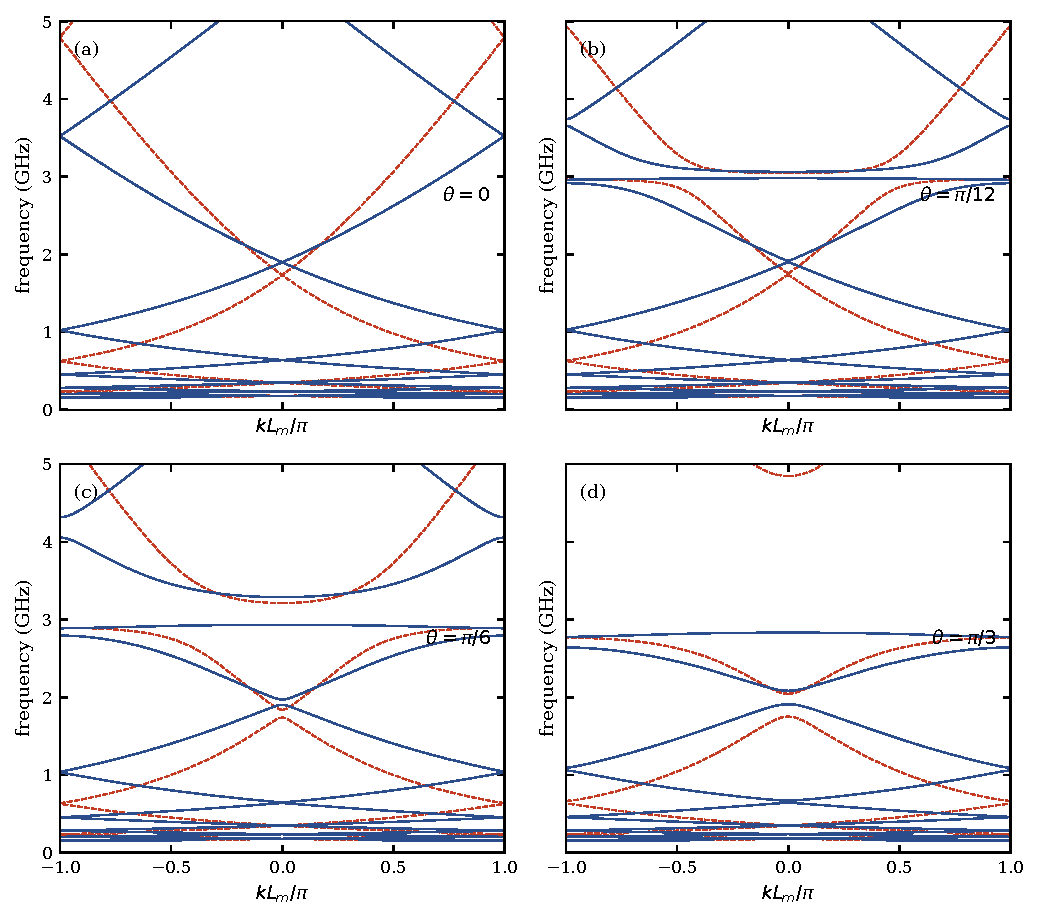
\includegraphics[width=\linewidth]{pwe/figure_01/output/figure_01.pdf}
\caption{Fig.~1 del paper calculada con el PWE ($\nu_e=\nu_m=3$~GHz, TE,
$m=3,4$).}
\label{fig:pwe1}
\end{figure}

\begin{figure}[H]
\centering
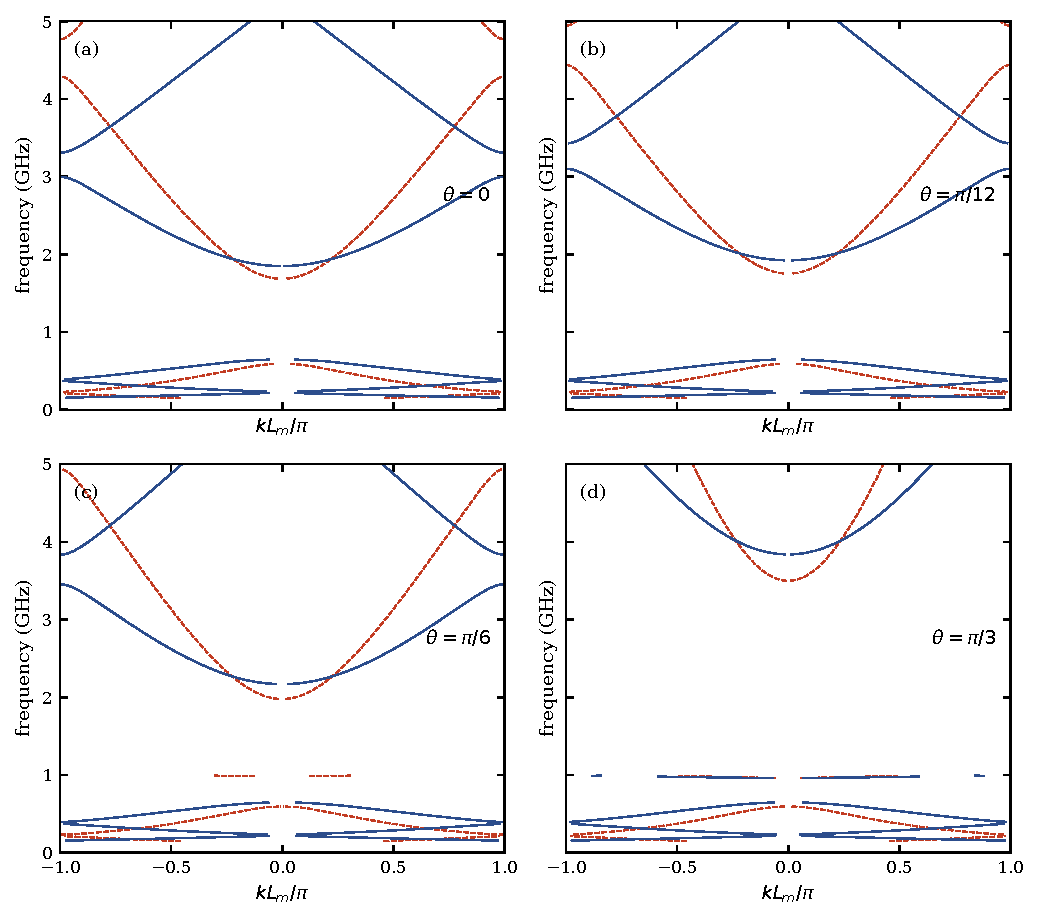
\includegraphics[width=\linewidth]{pwe/figure_03/output/figure_03.pdf}
\caption{Fig.~3 del paper calculada con el PWE ($\nu_e=3$~GHz, $\nu_m=1$~GHz).}
\label{fig:pwe3}
\end{figure}

\subsection{Figuras 2 y 4: número de subbandas}

Las Figs.~\ref{fig:pwe2} y~\ref{fig:pwe4} amplían la región de plasmón. El
número de subbandas detectado por el PWE es $F_{m-2}=1,2,3,5$ para
$m=3\dots6$ (Fig.~2) y $1,2$ para $m=3,4$ (Fig.~4), igual que con la TMM
(Tabla~\ref{tab:conteos}).

\begin{figure}[H]
\centering
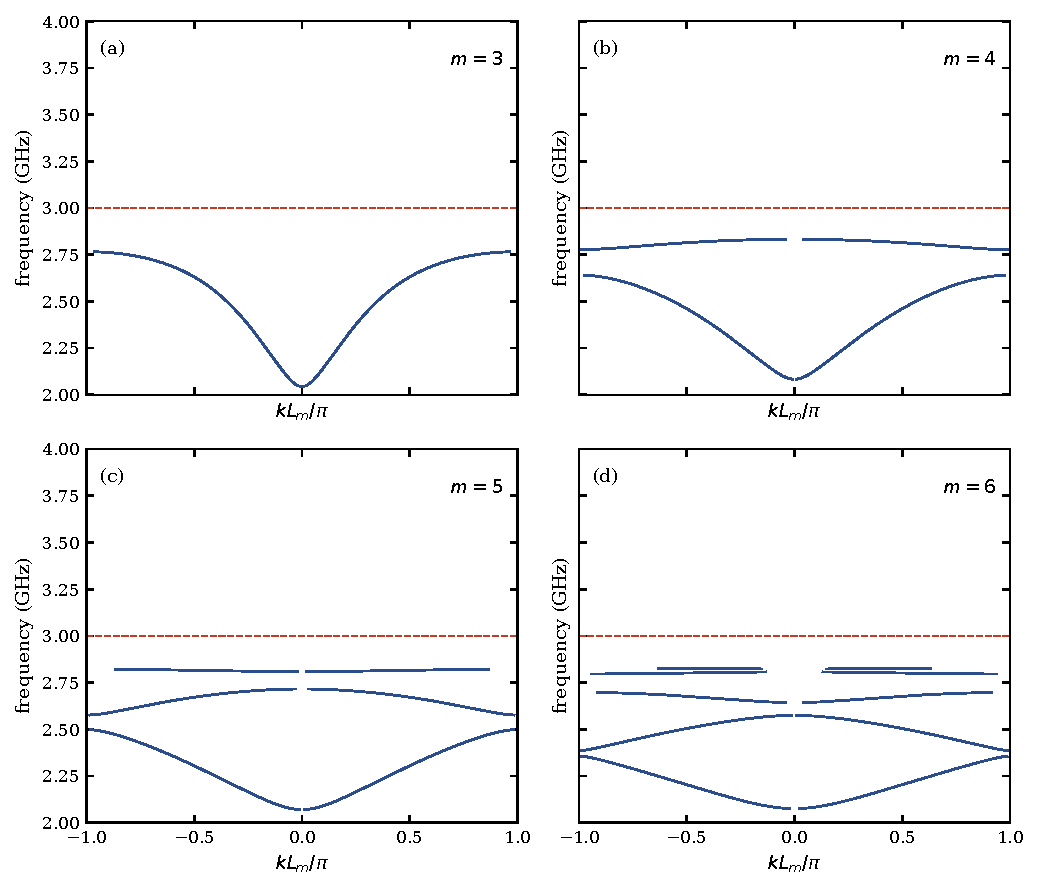
\includegraphics[width=\linewidth]{pwe/figure_02/output/figure_02.pdf}
\caption{Fig.~2 con el PWE: vecindad de $\nu_m=3$~GHz, $\theta=\pi/3$,
$m=3\dots6$.}
\label{fig:pwe2}
\end{figure}

\begin{figure}[H]
\centering
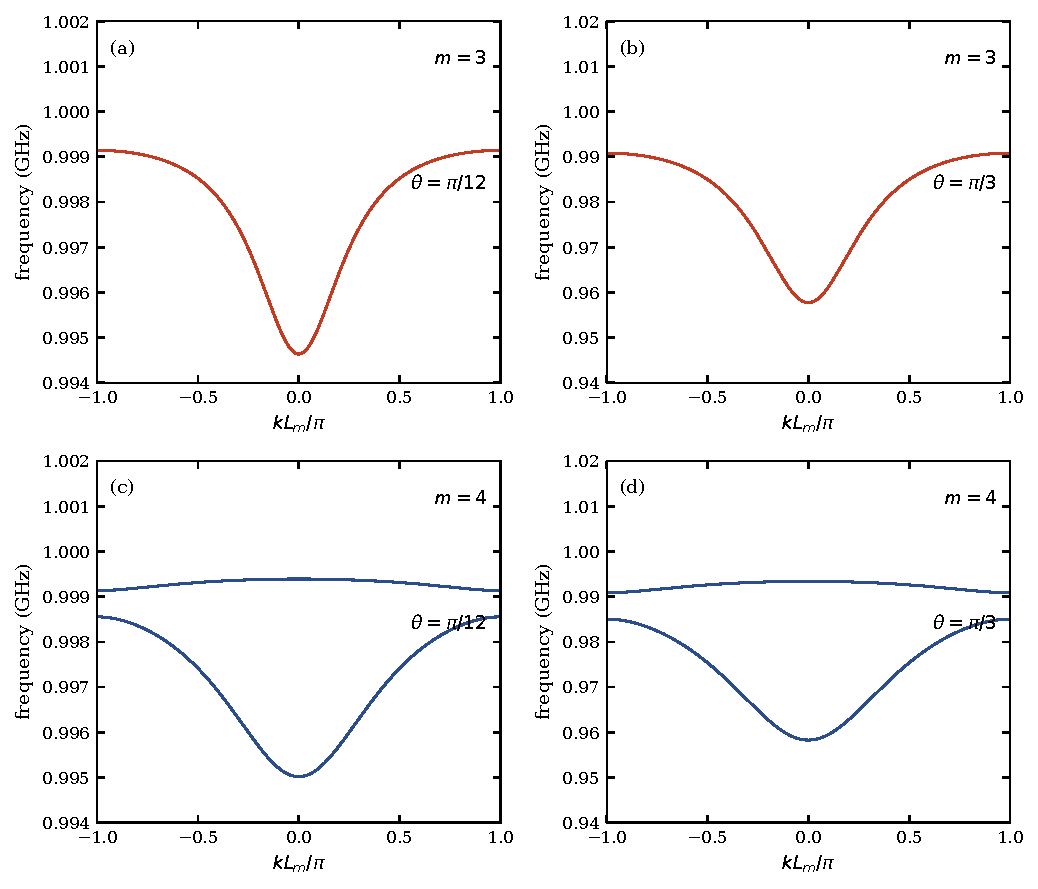
\includegraphics[width=\linewidth]{pwe/figure_04/output/figure_04.pdf}
\caption{Fig.~4 con el PWE: ampliación de los polaritones de la Fig.~3.}
\label{fig:pwe4}
\end{figure}

\begin{table}[H]
\centering
\caption{Acuerdo TMM--PWE en los barridos de las Figs.~1--4: error máximo en
$R$ dentro de las bandas, fracción de frecuencias con la misma clasificación
banda/gap y tiempos totales.}
\label{tab:dispersion}
\resizebox{\linewidth}{!}{\tabla{dispersion}}
\end{table}

\begin{table}[H]
\centering
\caption{Número de subbandas de plasmón-polaritón detectadas.}
\label{tab:conteos}
\tabla{mode_counts}
\end{table}

\subsection{Figuras 5 y 6: subbandas frente al orden y al ángulo}

La Fig.~\ref{fig:pwe5} reproduce la Fig.~5 del paper con el PWE para
$m=2\dots6$: los intervalos permitidos debajo de $\nu_m$, que se multiplican
siguiendo $F_{m-2}$ y se estrechan al crecer $m$. La Fig.~\ref{fig:pwe6}
reproduce los anchos de banda frente al ángulo (Fig.~6). Con el PWE se omite
$\theta=0$: allí las subbandas se concentran a menos de $10^{-5}$~GHz de $\nu_m$,
en la zona donde el método deja de ser fiable (Sec.~\ref{sec:validez}); la TMM sí
cubre ese ángulo. Los órdenes $m=7,8$ solo se calculan con la TMM por su costo
(Sec.~\ref{sec:costo}).

\begin{figure}[H]
\centering
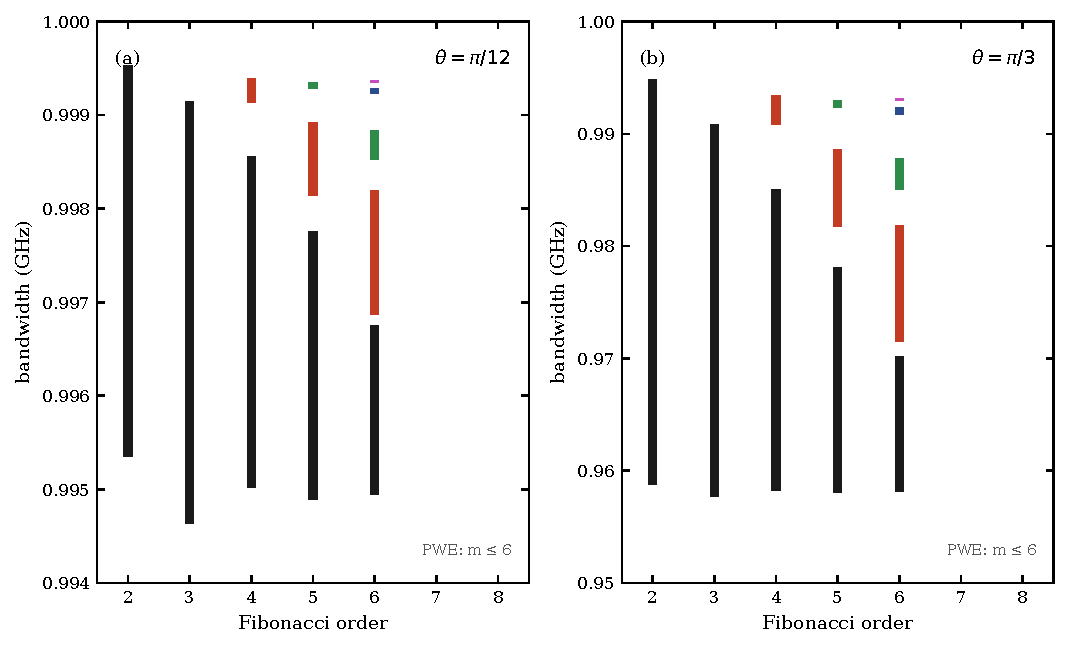
\includegraphics[width=\linewidth]{pwe/figure_05/output/figure_05.pdf}
\caption{Fig.~5 con el PWE: intervalos permitidos (segmentos) debajo de
$\nu_m=1$~GHz para $\theta=\pi/12$ y $\pi/3$, $m=2\dots6$.}
\label{fig:pwe5}
\end{figure}

\begin{figure}[H]
\centering
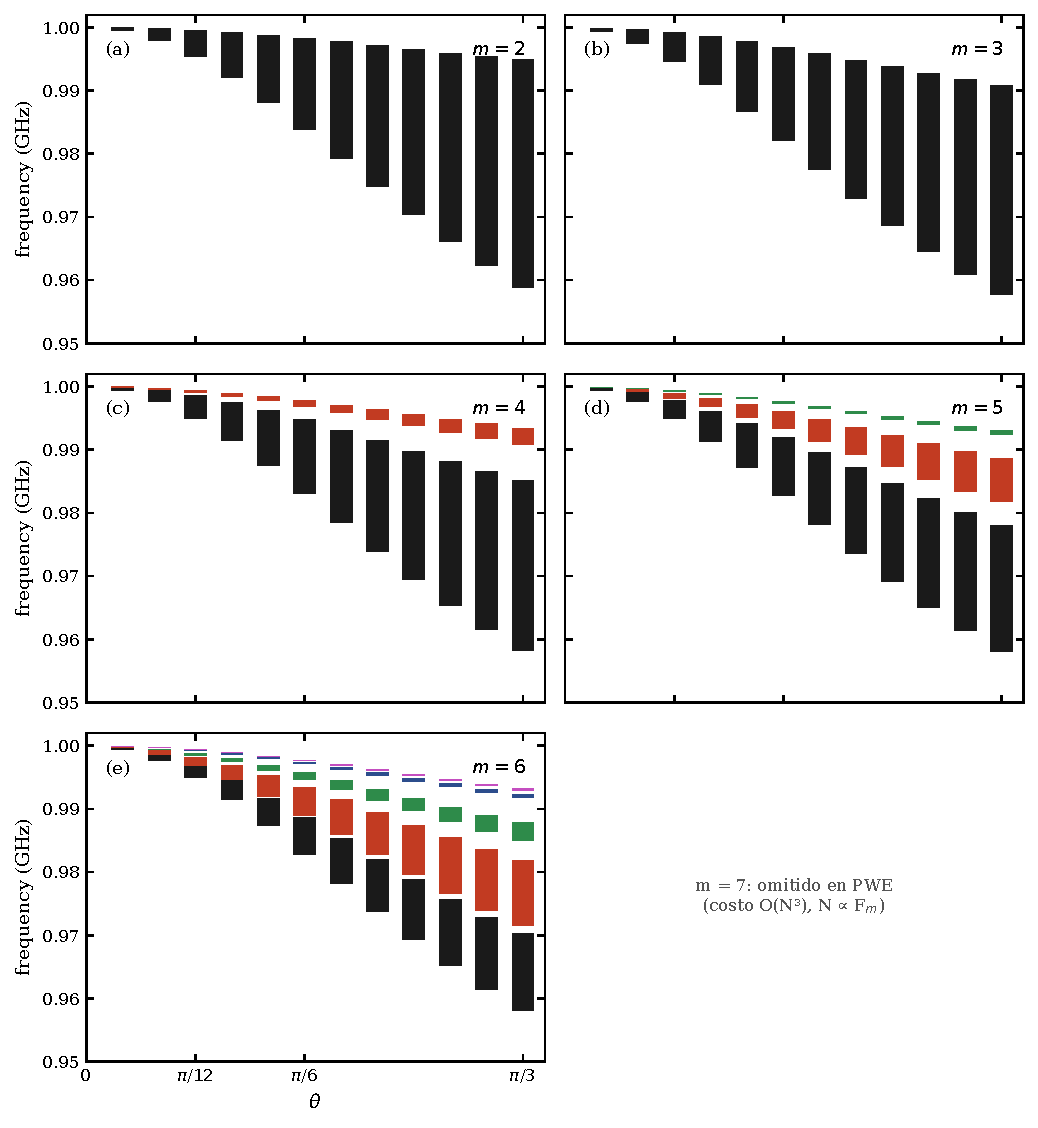
\includegraphics[width=\linewidth]{pwe/figure_06/output/figure_06.pdf}
\caption{Fig.~6 con el PWE: ancho de cada subbanda frente al ángulo de
incidencia, $m=2\dots6$, $\theta=5^\circ\dots60^\circ$.}
\label{fig:pwe6}
\end{figure}

\begin{table}[H]
\centering
\caption{Fig.~5: conteo de subbandas y error de los bordes del PWE respecto a la
TMM (misma malla y mismo localizador). $w$: ancho de la subbanda.}
\label{tab:fig5}
\resizebox{\linewidth}{!}{\tabla{figure_05}}
\end{table}

\begin{table}[H]
\centering
\caption{Fig.~6: casos por orden en los que TMM, PWE y $F_{m-2}$ coinciden, y
peores errores de borde y de ancho.}
\label{tab:fig6}
\tabla{figure_06}
\end{table}

%=====================================================================
\section{Convergencia, costo y límite de validez}\label{sec:costo}
%=====================================================================

\subsection{Convergencia con el número de ondas planas}

La Fig.~\ref{fig:book-conv} resume la convergencia en el cristal del libro y la
Fig.~\ref{fig:drude-conv} en la superred de Drude ($m=3,4,5$, TE y TM,
$\theta=\pi/6$). En el libro, Laurent converge como $N^{-1}$ y la regla inversa
como $N^{-3}$. En la superred la regla inversa mantiene la convergencia
$\sim N^{-3}$ para todos los órdenes y polarizaciones, mientras que Laurent se
estanca en errores de $10^{-2}$ a $1$ y, en TM, llega a errores de $10^2$ o más
con pocas ondas planas: allí $\varepsilon_B$, que es la función dentro de la
derivada, cambia de signo en la ventana.

\begin{figure}[H]
\centering
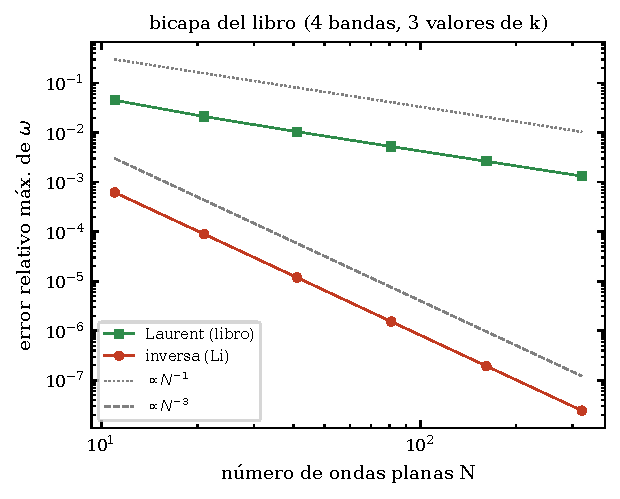
\includegraphics[width=0.8\linewidth]{pwe/convergence/output/book_convergence.pdf}
\caption{Cristal del libro: error relativo máximo de las cuatro primeras bandas
(tres valores de $k$) frente a $N$, con las reglas de Laurent e inversa.}
\label{fig:book-conv}
\end{figure}

\begin{figure}[H]
\centering
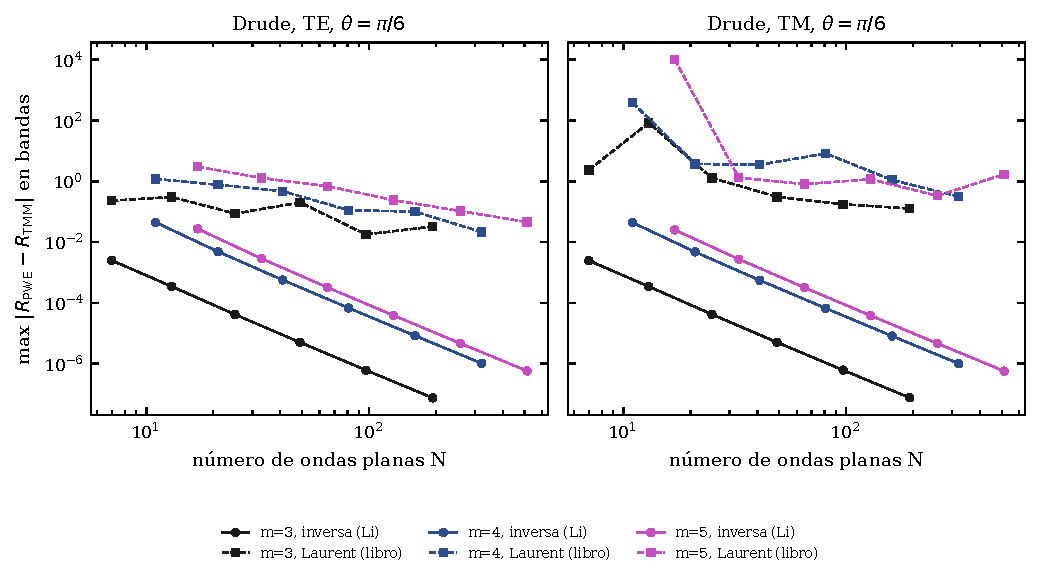
\includegraphics[width=0.8\linewidth]{pwe/convergence/output/drude_convergence.pdf}
\caption{Superred de Drude (parámetros de la Fig.~5 del paper, $\theta=\pi/6$,
60 frecuencias entre 0.3 y 5~GHz): error máximo en $R$ dentro de las bandas
frente a la TMM según $N$, para $m=3,4,5$, en TE y TM, con ambas reglas.}
\label{fig:drude-conv}
\end{figure}

\subsection{Costo}

Cada frecuencia exige los autovalores de una matriz $2N\times2N$, es decir
$O(N^3)$ operaciones con $N=2hF_m+1$. Como $F_m$ crece como $\phi^m$
($\phi$ el número áureo), el costo crece como $\phi^{3m}$. La TMM, en cambio,
multiplica $F_m$ matrices $2\times2$ (o aplica la recurrencia $T_m=T_{m-2}T_{m-1}$).
La Tabla~\ref{tab:costo} y la Fig.~\ref{fig:costo} cuantifican la diferencia: de
entre tres y cinco órdenes de magnitud por frecuencia, y la razón crece con $m$.
El anexo \textit{Comparación TMM vs PWE} amplía este análisis con mediciones en
un núcleo. El tiempo del PWE crece como $N^{\EffAlphaShort}$ (\EffPweLast{} por
frecuencia con $m=\EffPweLastM$), mientras que la TMM por recurrencia se mantiene en
$\sim\!\EffTmmRecMax~\mu$s hasta $m=\EffTmmMaxM$. Para un error de $\EffWpBestErr$
el PWE necesita \EffWpBestTime{} por frecuencia, y la TMM llega al redondeo de la
máquina en microsegundos. Las seis figuras del paper cuestan \EffFigTmmTotal{} con
la TMM y unas \EffFigPweTotal{} con el PWE. De ahí se concluye que la TMM
es el método óptimo para la superred 1D.

\begin{table}[H]
\centering
\caption{Costo por frecuencia y precisión del PWE frente a la TMM.}
\label{tab:costo}
\resizebox{\linewidth}{!}{\tabla{cost}}
\end{table}

\begin{figure}[H]
\centering
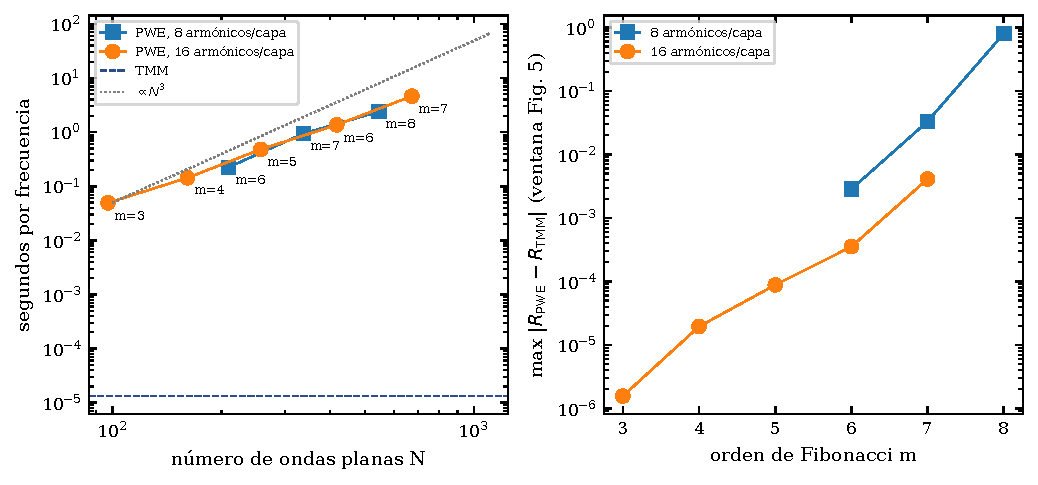
\includegraphics[width=0.85\linewidth]{pwe/convergence/output/cost_and_accuracy.pdf}
\caption{Tiempo por frecuencia y error máximo en $R$ según el orden de Fibonacci.}
\label{fig:costo}
\end{figure}

\subsection{Límite de validez cerca de $\nu_m$}\label{sec:validez}

Justo debajo de $\nu_m$, $\mu_B\to0^-$ y la onda es muy evanescente en las capas
B. En los gaps profundos $|R|$ llega a $10^4$ o más ($|\mathrm{Im}\,kL_m|\gtrsim10$):
el modo seleccionado está exponencialmente amortiguado y el truncamiento de
Fourier ya no lo representa bien. A menos de $\sim\!10^{-7}$--$2\times10^{-6}$~GHz
de $\nu_m$ el PWE produce oscilaciones de $R$ que cruzan $|R|=1$ y parecerían
bandas (Fig.~\ref{fig:validez}). No son físicas: al aumentar $N$ se desplazan
y $|R|$ cambia en órdenes de magnitud. Por eso: (i) las mallas del PWE terminan a
$10^{-7}$~GHz de $\nu_m$, y (ii) cada banda se valida con $1.5N$ ondas planas
(Sec.~\ref{sec:bordes}). La Tabla~\ref{tab:fig5} muestra que tras esa validación
el conteo coincide con la TMM en todos los casos.

\begin{figure}[H]
\centering
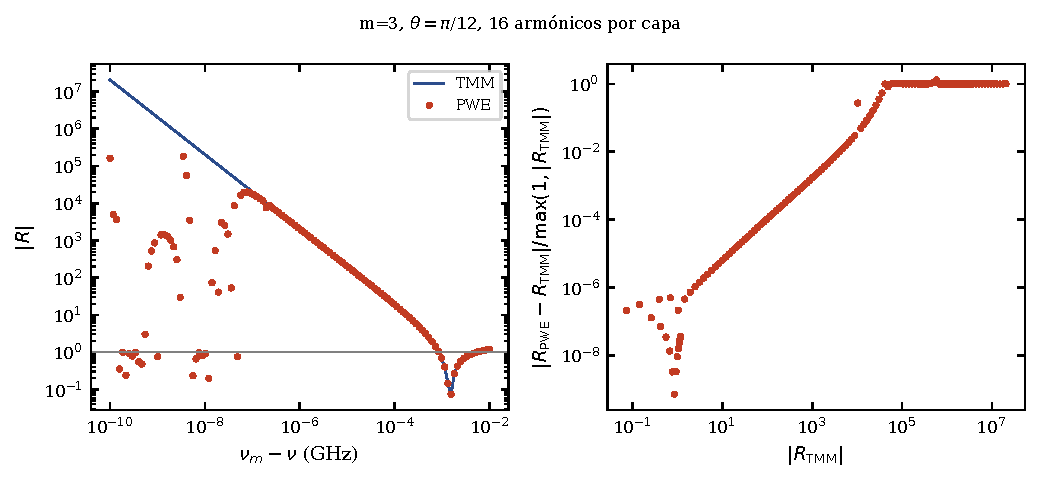
\includegraphics[width=0.85\linewidth]{pwe/convergence/output/validity_near_nu_m.pdf}
\caption{Semitraza cerca de $\nu_m$ calculada con la TMM y con el PWE para varios
$N$. Lejos del polo las curvas coinciden; a menos de $\sim\!10^{-6}$~GHz el PWE
diverge de la TMM y depende de $N$.}
\label{fig:validez}
\end{figure}

%=====================================================================
\section{Conclusiones}
%=====================================================================

\begin{enumerate}
\item El PWE del libro se extendió a la celda de Fibonacci con la
generalización~\eqref{eq:fourier} de la ec.~(4.38) y reproduce los resultados
del capítulo 1D (bandas, síntesis, campo y bandas fuera del eje con Brewster).
\item La forma $\omega(k)$ no es adecuada para metamateriales de Drude: el
problema se vuelve cuadrático en $\omega^2$ y aparece contaminación espectral
acumulada en $\nu_m$.
\item La forma $k(\omega)$, un QEP en $k$ con la regla inversa de Li, evita ese
problema, da directamente la semitraza $R=\cos kL_m$ del paper y coincide con
la TMM en todas las figuras: mismo conteo $F_{m-2}$ de subbandas y bordes con
errores relativos de ancho menores que $10^{-5}$.
\item La regla de factorización es esencial: con la regla de Laurent del libro
el error con Drude se estanca entre $10^{-2}$ (TE) y $10^{-1}$--$1$ (TM), mientras
que con la regla inversa decrece como $N^{-3}$.
\item El PWE cuesta entre tres y cinco órdenes de magnitud más por frecuencia que la TMM
(\EffFigTmmTotal{} frente a $\approx$\EffFigPweTotal{} para las seis figuras en un
núcleo), su costo
crece como $\phi^{3m}$ frente a $O(m)$, y falla en los gaps profundos junto a
$\nu_m$. Por tanto la TMM es el método óptimo y sigue siendo el método
de producción del proyecto, y el PWE queda como verificación independiente y
como base para la extensión a dos dimensiones, donde la TMM ya no se aplica.
\end{enumerate}

%=====================================================================
\appendix
\section{Correspondencia con el código y reproducibilidad}\label{app:codigo}
%=====================================================================

\begin{table}[H]
\centering
\caption{Ecuaciones y módulos (rutas relativas a \code{solvers/pwe/} salvo las de \code{analysis/} y \code{comparison/}).}
\begin{tabular}{ll}
\toprule
Ecuación & Implementación \\
\midrule
\eqref{eq:fourier}, \eqref{eq:toeplitz} & \code{fourier.py}: \code{cell\_fourier}, \code{toeplitz\_matrix} \\
\eqref{eq:maestra} (no dispersivo) & \code{eigenfrequency.py}: \code{nondispersive\_bands} \\
\eqref{eq:qep-omega} (Drude, $\omega(k)$) & \code{eigenfrequency.py}: \code{drude\_qep\_frequencies\_ghz} \\
\eqref{eq:qep-k}, \eqref{eq:companion} & \code{bloch.py}: \code{qep\_matrices}, \code{bloch\_eigenvalues} \\
\eqref{eq:rpwe} & \code{bloch.py}: \code{select\_bloch\_wavevector}, \code{solve\_bloch} \\
barrido & \code{solver.py}: \code{PWESolver}; \code{semitrace.py}: \code{SemitraceEvaluator} \\
convergencia & \code{convergence.py}: \code{check\_harmonic\_convergence} \\
bordes y validación & \code{analysis/band\_edges.py}: \code{locate\_bands}, \code{validate\_bands} \\
comparación & \code{comparison/compare.py}: \code{compare\_scans} \\
\bottomrule
\end{tabular}
\end{table}

El núcleo del solver $k(\omega)$ (\code{solvers/pwe/bloch.py}) es:
\begin{lstlisting}
t_chi = cell.toeplitz(chi_a, chi_b)            # [[χ]]
t_inv_chi = cell.toeplitz(1 / chi_a, 1 / chi_b)  # [[1/χ]]
p = np.linalg.inv(t_chi)                       # regla inversa: P = [[χ]]^-1
f = kappa**2 * cell.toeplitz(psi_a, psi_b) - q2 * t_inv_chi
a1 = p @ g + g @ p
a0 = g @ p @ g - f
companion = [[0, I], [-t_chi @ a0, -t_chi @ a1]]   # P^-1 = [[χ]]
k_tilde = select(np.linalg.eigvals(companion))  # min |Im k̃|, |Re k̃| <= 1.25π
r = np.cos(k_tilde).real
\end{lstlisting}

\paragraph{Reproducir.} Desde la raíz del proyecto:
\begin{lstlisting}[language=bash]
python scripts/tmm/run_all.py         # results/tmm/
python scripts/pwe/run_all.py         # results/pwe/   (PWE_WORKERS=n limita procesos)
python scripts/comparison/run_all.py  # results/comparison/ y tablas LaTeX
make pwe-docs                         # este documento y el anexo
\end{lstlisting}

\begin{thebibliography}{9}
\bibitem{prb2010} E. Reyes-Gómez, D. Mogilevtsev, S. B. Cavalcanti, C. A. A. de
Carvalho y L. E. Oliveira, ``Plasmon polaritons in photonic superlattices
containing a left-handed material'', Phys.\ Rev.\ B \textbf{81}, 153101 (2010).
\bibitem{sukhoivanov} I. A. Sukhoivanov e I. V. Guryev, \textit{Photonic
Crystals: Physics and Practical Modeling}, Springer Series in Optical Sciences
152 (Springer, 2009), cap.~4: ``Band Structure Computation of 1D Photonic
Crystals''. Copia local en \code{referencias/metodo\_ondas\_planas/PWE-Method-1D.pdf}; cuaderno
\code{referencias/metodo\_ondas\_planas/PWE-1d.ipynb}.
\bibitem{li1996} L. Li, ``Use of Fourier series in the analysis of
discontinuous periodic structures'', J.\ Opt.\ Soc.\ Am.\ A \textbf{13},
1870--1876 (1996).
\bibitem{tisseur} F. Tisseur y K. Meerbergen, ``The quadratic eigenvalue
problem'', SIAM Review \textbf{43}, 235--286 (2001).
\bibitem{tip} A. Tip, A. Moroz y J.-M. Combes, ``Band structure of absorptive
photonic crystals'', J.\ Phys.\ A \textbf{33}, 6223 (2000).
\bibitem{joannopoulos} J. D. Joannopoulos, S. G. Johnson, J. N. Winn y R. D.
Meade, \textit{Photonic Crystals: Molding the Flow of Light}, 2.ª ed.
(Princeton University Press, 2008).
\end{thebibliography}

\end{document}
